This component diagram, as the title suggest, is designed to deeply analyze the atomic components of the application server, since they are the core of the whole architecture in terms of complexity of computations and relevance in assolving functional requirements. \\
Since this diagram aims to explain almost every logical component and its interactions, it is quite complex and difficult to be read and understood, for this reason we append to it some tables to specify both the interactions and the role of each component. \\



\begin{figure} 
\begin{center}

\makebox[\textwidth]{%
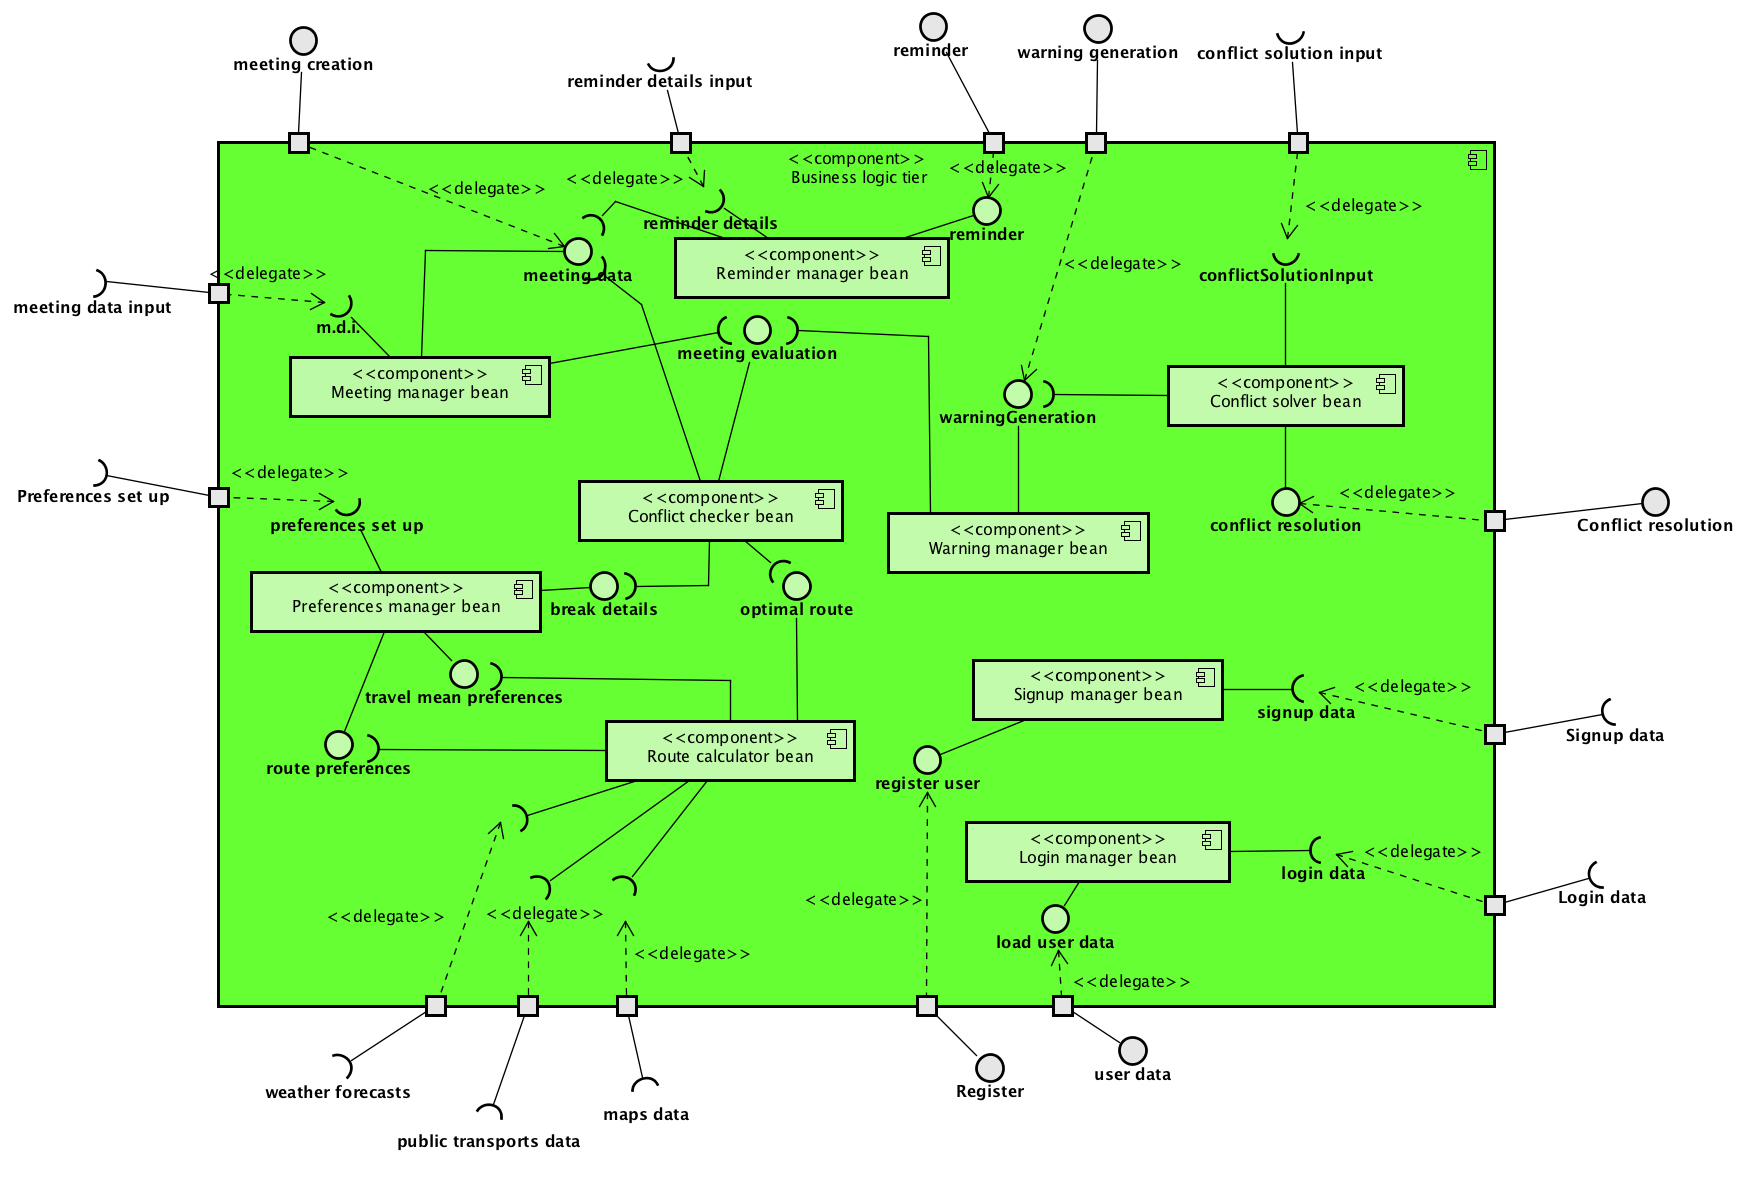
\includegraphics[width=1.5\linewidth]{images/LLcomponentdiagram} 
}
\caption{Low-level component diagram} 
\label{fig:llcomponentdiagram} 


\end{center}
\end{figure} 
